\documentclass[UTF8]{ctexbeamer}

\usetheme{Boadilla}

\usecolortheme{rose}

\usepackage{graphicx}
\usepackage{color}
\usepackage{tikz}
\usepackage{xcolor}
\usepackage{pgfplots}
\usepackage{listings}
\usepackage{amsmath}

\definecolor{light-gray}{gray}{0.95}
\newcommand{\code}[1]{\colorbox{light-gray}{\texttt{#1}}}

\pgfplotsset{width=7cm,compat=1.6}
\usefonttheme[onlymath]{serif}

\newfontfamily\courier{Courier New}
\lstset{linewidth=1.1\textwidth,
	numbers=left,
	basicstyle=\small\courier,
	numberstyle=\tiny\courier,
	keywordstyle=\color{blue}\courier,
	commentstyle=\it\color[cmyk]{1,0,1,0}\courier, 
	stringstyle=\it\color[RGB]{128,0,0}\courier,
	breaklines,
	extendedchars=false, 
	xleftmargin=2em,xrightmargin=2em, aboveskip=1em,
	tabsize=4, 
	basicstyle=\small\courier
}

\tikzstyle{myBlock}=[draw, fill=blue!30!white, minimum size=0.5in, node distance=2.25in]
\usetikzlibrary{arrows.meta}
\tikzstyle{myPath} = [-{Latex[length=2mm,width=2mm]}, line width=0.4mm]


\begin{document}

\title{计算机系统结构实验五}
\author{\songti 于海鑫}
\institute{2017211240}

\date{\today}

\frame{\titlepage}

\section{指令调度}
\begin{frame}
\frametitle{执行程序:步骤}
\begin{itemize}
    \item 启动 MIPSsim。
    \item 用 MIPSsim 的 ``文件'' $\rightarrow$ ``载入程序'' 选项来加载 \code{schedule.s}(在模拟器所在文件夹下的“样例程序”文件夹中)。
    \item 关闭定向功能,这是通过 ``配置'' $\rightarrow$ ``定向'' 选项来实现的。
    \item  执行所载入的程序,通过查看统计数据和时钟周期图,找出并记录程序执行过程中各种冲突发生的次数,发生冲突的指令组合以及程序执行的总时钟周期数。
\end{itemize}
\end{frame}

\begin{frame}
    \frametitle{执行程序:统计数据}
    \begin{itemize}
        \item 总执行周期:33
        \item RAW停顿:16		占周期总数的百分比:48.48485\%
        \\ 其中:load停顿:6		占所有RAW停顿的百分比:37.5\%
        \item WAW停顿:0		占周期总数的百分比:0\%
        \item 结构停顿:0		占周期总数的百分比:0\%
        \item 控制停顿:0		占周期总数的百分比:0\%
        \item 自陷停顿:1		占周期总数的百分比:3.030303\%
        \item 停顿周期总数:17	占周期总数的百分比:51.51515\%
    \end{itemize}
\end{frame}

\begin{frame}
    \frametitle{执行程序:统计数据}
    \begin{figure}[H]
        \centering
        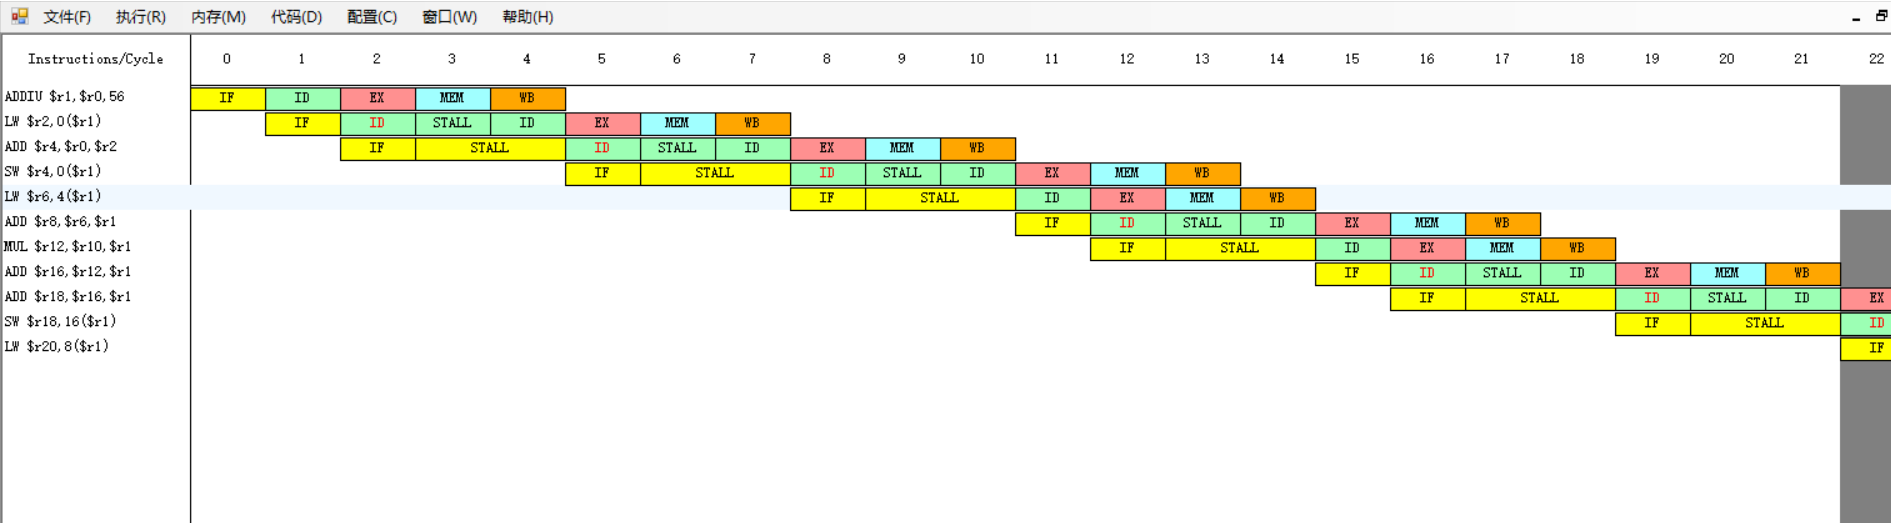
\includegraphics[width=\textwidth]{fig/schedule.png}
      \end{figure}
\end{frame}

\begin{frame}
    \frametitle{执行程序:统计数据}
    \begin{itemize}
        \item ADDIU \$1, \$0, 56 和 LW \$r2,0(\$r1)
        \item LW \$r2,0(\$r1) 和 ADD \$r4,\$r0,\$r2
        \item ADD \$r4,\$r0,\$r2 和 SW \$r4,0(\$r1)
        \item LW \$r6,4(\$r1) 和 ADD \$r8,\$r6,\$r1
        \item MUL \$r12,\$r10,\$r1 和 ADD \$r16,\$r12,\$r1
        \item ADD \$r16,\$r12,\$r1 和 ADD \$r18,\$r16,\$r1
        \item ADD \$r18,\$r16,\$r1 和 SW \$r18,16(\$r1)
        \item MUL \$r22,\$r20,\$r14 和 MUL \$r24,\$r26,\$r14
    \end{itemize}
\end{frame}

\begin{frame}
    \frametitle{静态调度}
    \centering 核心思路:在不改变程序运行结果的情况下,尽可能将不相关的指令安插在由冲突的指令中间
\end{frame}

\begin{frame}[fragile]
    \frametitle{静态调度:原始程序}
    \begin{lstlisting}
.text
main:
ADDIU  $r1,$r0,A
LW     $r2,0($r1)
ADD    $r4,$r0,$r2
SW     $r4,0($r1)
LW     $r6,4($r1)
ADD    $r8,$r6,$r1
MUL    $r12,$r10,$r1
ADD    $r16,$r12,$r1
ADD    $r18,$r16,$r1
SW     $r18,16($r1)
LW     $r20,8($r1)
MUL    $r22,$r20,$r14
MUL    $r24,$r26,$r14
TEQ    $r0,$r0
    \end{lstlisting}
\end{frame}

\begin{frame}[fragile]
    \frametitle{静态调度:调度结果}
    \begin{lstlisting}
.text
main:
ADDIU  $r1,$r0,A
MUL    $r24,$r26,$r14
LW     $r2,0($r1)
MUL    $r12,$r10,$r1
LW     $r6,4($r1)
ADD    $r4,$r0,$r2
ADD    $r16,$r12,$r1
LW     $r20,8($r1)
SW     $r4,0($r1)
ADD    $r18,$r16,$r1
ADD    $r8,$r6,$r1
MUL    $r22,$r20,$r14
SW     $r18,16($r1)
TEQ    $r0,$r0
    \end{lstlisting}
\end{frame}

\begin{frame}
    \frametitle{静态调度:统计数据}
    \begin{itemize}
        \item 总执行周期:18
        \item RAW停顿:1		占周期总数的百分比:5.555555\%
        \\ 其中:load停顿:0		占所有RAW停顿的百分比:0\%
        \item WAW停顿:0		占周期总数的百分比:0\%
        \item 结构停顿:0		占周期总数的百分比:0\%
        \item 控制停顿:0		占周期总数的百分比:0\%
        \item 自陷停顿:1		占周期总数的百分比:5.555555\%
        \item 停顿周期总数:2	占周期总数的百分比:11.11111\%
    \end{itemize}
\end{frame}

\begin{frame}
    \frametitle{静态调度:统计数据}
    \begin{figure}[H]
        \centering
        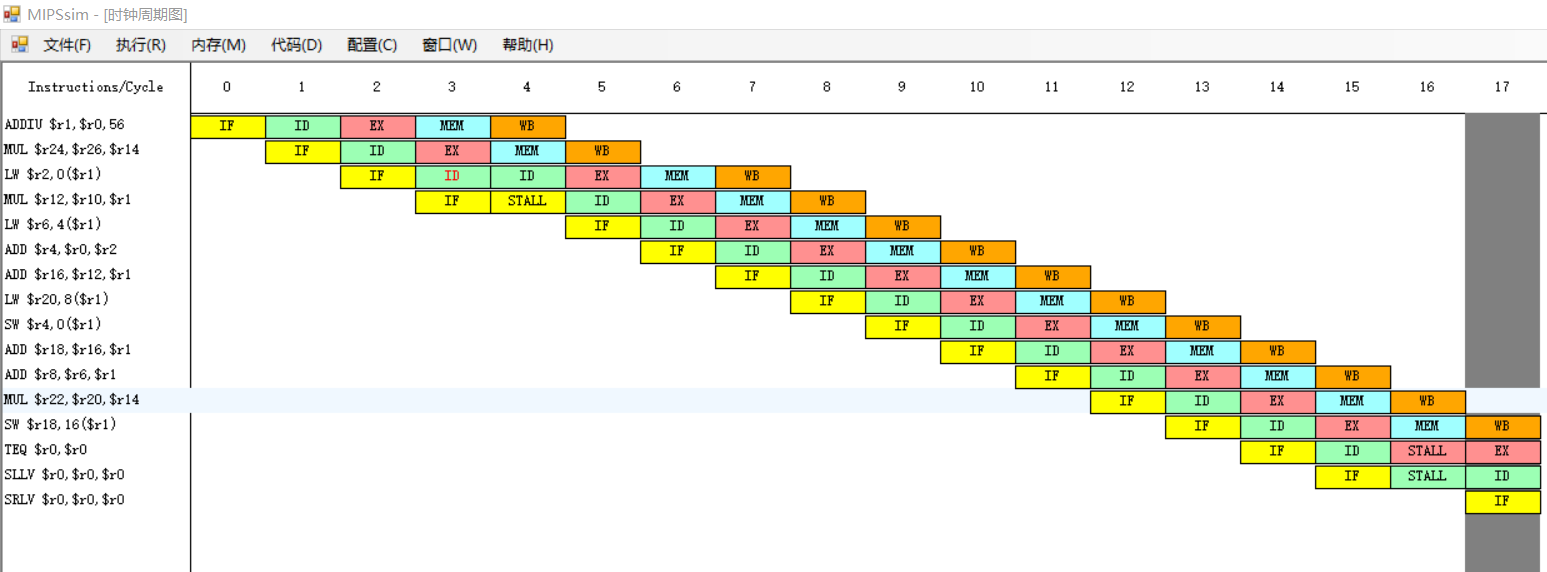
\includegraphics[width=\textwidth]{fig/after-schedule.png}
      \end{figure}
\end{frame}

\section{延迟分支}
\begin{frame}
    \frametitle{执行程序:步骤}
    \begin{itemize}
        \item 在 MIPSsim 中载入 \code{branch.s} 样例程序(在本模拟器目录的“样例程序”文件夹中。
          \item 关闭延迟分支功能。这是通过在“配置” $\rightarrow$ “延迟槽”选项来实现的。
          \item 执行该程序,观察并记录发生分支延迟的时刻,记录该程序执行的总时钟周期数。
    \end{itemize}
\end{frame}

\begin{frame}
    \frametitle{执行程序:统计数据}
    \centering 总执行周期:38

    \centering 第 14,29 周期发生了分支延迟
\end{frame}

\begin{frame}
    \frametitle{执行程序:统计数据}
    \begin{figure}[H]
        \centering
        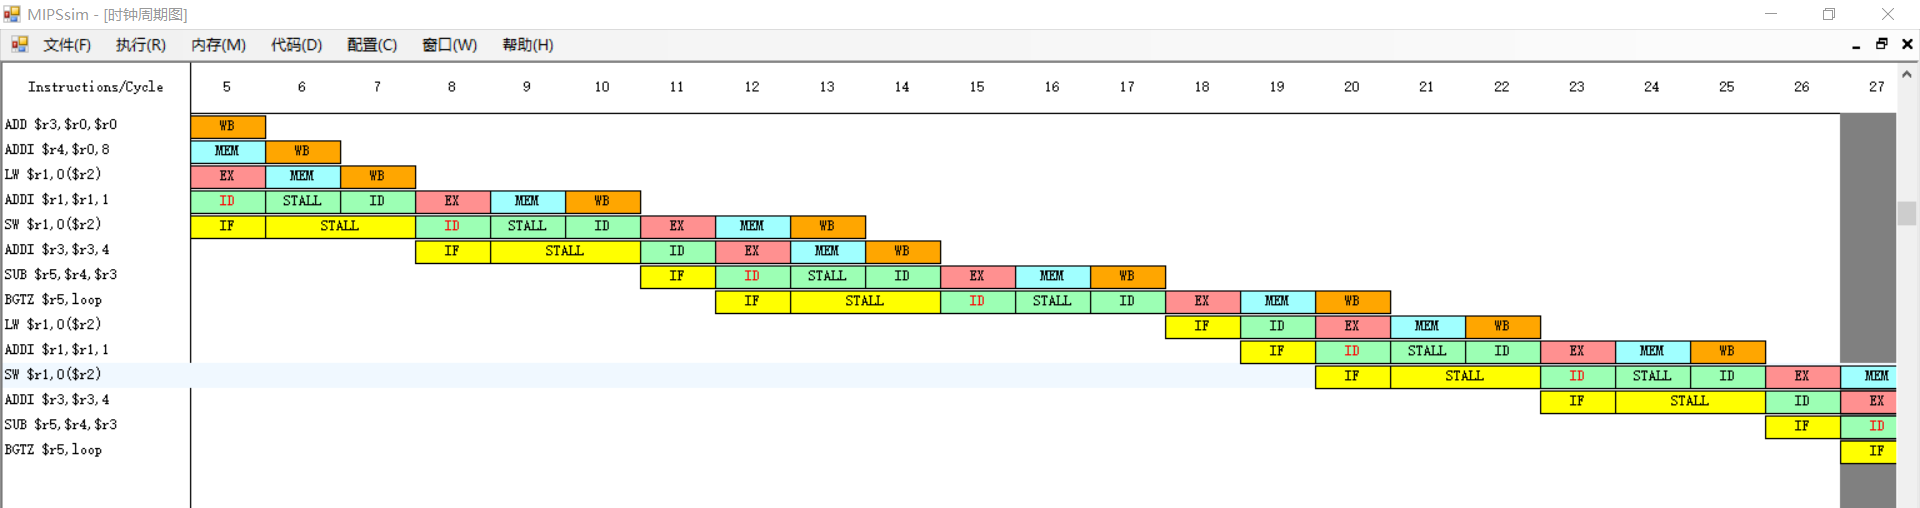
\includegraphics[width=\textwidth]{fig/branch.png}
      \end{figure}
\end{frame}

\begin{frame}[fragile]
    \frametitle{指令调度:原始程序}
    \begin{lstlisting}
.text
main:
ADDI  $r2,$r0,1024
ADD   $r3,$r0,$r0
ADDI  $r4,$r0,8
loop:  
LW    $r1,0($r2)
ADDI  $r1,$r1,1
SW    $r1,0($r2)
ADDI  $r3,$r3,4
SUB   $r5,$r4,$r3
BGTZ  $r5,loop
ADD   $r7,$r0,$r6
TEQ   $r0,$r0
    \end{lstlisting}
\end{frame}

\begin{frame}[fragile]
    \frametitle{指令调度:调度结果}
    \begin{lstlisting}
.text
main:
ADDI  $r2,$r0,1024
ADD   $r3,$r0,$r0
ADDI  $r4,$r0,8
LW    $r1,0($r2)
loop:  
ADDI  $r1,$r1,1
ADDI  $r3,$r3,4
SUB   $r5,$r4,$r3
SW    $r1,0($r2)
BGTZ  $r5,loop
LW    $r1,0($r2)

ADD   $r7,$r0,$r6
TEQ   $r0,$r0
    \end{lstlisting}
\end{frame}

\begin{frame}
    \frametitle{执行程序:统计数据}
    \centering 总执行周期:31
\end{frame}

\begin{frame}
    \frametitle{执行程序:统计数据}
    \begin{figure}[H]
        \centering
        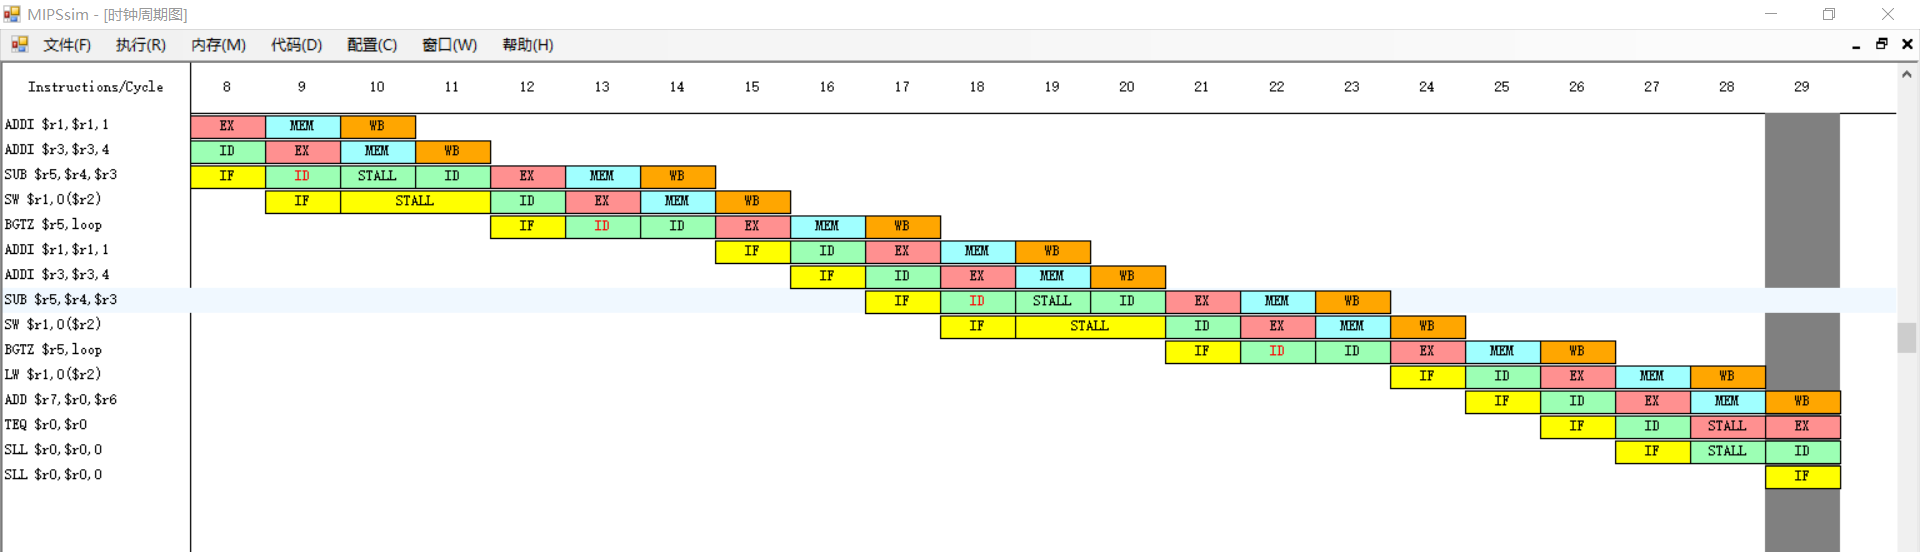
\includegraphics[width=\textwidth]{fig/delayed-branch.png}
      \end{figure}
\end{frame}

\begin{frame}
    \begin{center}
        \Huge Thank You
    \end{center}
\end{frame}

\end{document}